\documentclass{article}
\usepackage[top=20mm, bottom=20mm]{geometry}
\usepackage{multicol}
\usepackage{graphicx}
\usepackage[center]{caption}

\title{MATH321 - Assignment 3}
\author{Erdal Sidal Dogan\\ MEF University\\ \#041701076}
\begin{document}
	\maketitle
	\section{Q1}
	\subsection{Formal Definition}
	$Q = \{Q_0, Q_1, Q_2, Q_3, Q_4, Q_5, Q_6, Q_7\}$\\
	$\Sigma = \{A, C, D, X, Y, Z\}$\\
	$\Gamma =  \{A, D, X, Y, Z\}$\\
	$\delta: $ See below\\
	$q_0 = Q_0$\\
	$q_{accept} = \{ Q_7\}$\\
	
	%\subsection{Transition Function $(\delta)$} \label{tf}
	\begin{table}[h]
		\centering
			\begin{tabular}{c|c|c|c|c|c|c}
				$\delta$ & A & C & D & X & Y & Z \\
				\hline
				$Q_0$ & $(Q_1, X, R)$ & & & & $(Q_4, Y, R)$ & \\
				$Q_1$ & $(Q_1, A, R)$  & & $(Q_2, Y, R)$ & & $(Q_1, Y, R)$ & \\
				$Q_2$ & & $(Q_3, Z, L)$ & $(Q_2, D, R)$ & & & $(Q_2, Z, R)$ \\
				$Q_3$ & $(Q_3, A, L)$ & & $(Q_3, D, L)$ & $(Q_0, X, R)$ & $(Q_3, Y, L)$ & $(Q_3, Z, L)$ \\
				$Q_4$ & & & $(Q_5, Y, R)$ & & $(Q_4, Y, R)$&$(Q_7, Z, L)$ \\
				$Q_5$ & & $(Q_6, Z, L)$ & $(Q_5, D, R)$ & & &$(Q_5, Z, R)$ \\
				$Q_6$ & & & $(Q_6, D, L)$ & & $(Q_4, Y, R)$ & $(Q_6, Z, L)$ \\
				$Q_7$ & & & & & & \\
		\end{tabular}
		\caption{Transition Function Table}
	\end{table}
	
	\subsection{Configuration for 'AADDDCCCCCC'}
	\begin{multicols}{3}
		\begin{minipage}{0.33\textwidth}
			$q_0$AADDDCCCCCC\\
			X$q_1$ADDDCCCCCC\\
			XA$q_1$DDDCCCCCC\\
			XAY$q_2$DDCCCCCC\\
			XAYD$q_2$DCCCCCC\\
			XAYDD$q_2$CCCCCC\\
			XAYD$q_3$DZCCCCC\\
			\vdots \\
			$q_3$XAYDDZCCCCC\\
			X$q_0$AYDDZCCCCC\\

		\end{minipage}
		
		\begin{minipage}{0.33\textwidth}
			XX$q_1$YDDZCCCCC\\
			XXY$q_1$DDZCCCCC\\
			XXYY$q_2$DZCCCCC\\
			XXYYD$q_2$ZCCCCC\\
			XXYYDZ$q_2$CCCCC\\
			XXYYD$q_3$ZZCCCC\\
			\vdots \\
			X$q_3$XYYDZZCCCC\\
			XX$q_0$YYDZZCCCC\\
			XXY$q_4$YDZZCCCC\\

			
		\end{minipage}
		
		\begin{minipage}{0.33\textwidth}
			XXYY$q_4$DZZCCCC\\
			XXYYY$q_5$ZZCCCC\\
			XXYYYZ$q_5$ZCCCC\\
			XXYYYZZ$q_5$CCCC\\
			XXYYYZ$q_6$ZZCCC\\
			XXYYY$q_6$ZZZCCC\\
			XXYY$q_6$YZZZCCC\\
			XXYYY$q_4$ZZZCCC\\
			XXYY$q_7$YZZZCCC\\
		\end{minipage}
	\end{multicols}
	\newpage
	\subsection{Configuration for 'AAADDC'}
	\begin{multicols}{3}
		\begin{minipage}{0.33\textwidth}
			$q_0$AAADDC\\
			X$q_1$AADDC\\
			XA$q_1$ADDC\\
			XAA$q_1$DDC\\
			XAAY$q_2$DC\\
			XAAYD$q_2$C\\
		\end{minipage}
		
		\begin{minipage}{0.33\textwidth}
			XAA$q_3$YDZ\\
			XA$q_3$AYDZ\\
			X$q_3$AAYDZ\\
			$q_3$XAAYDZ\\
			X$q_0$AAYDZ\\
			XX$q_1$AYDZ\\
		\end{minipage}
	
		\begin{minipage}{0.33\textwidth}
			XXA$q_1$YDZ\\
			XXAY$q_1$DZ\\
			XXAY$q_1$DZ\\
			XXAYY$q_2$Z\\
			XXAYYZ$q_2$B\\
		\end{minipage}
	\end{multicols}

	\section{Q2}
	\subsection{Turing Machine}
	\begin{center}
		\vspace{2em}
		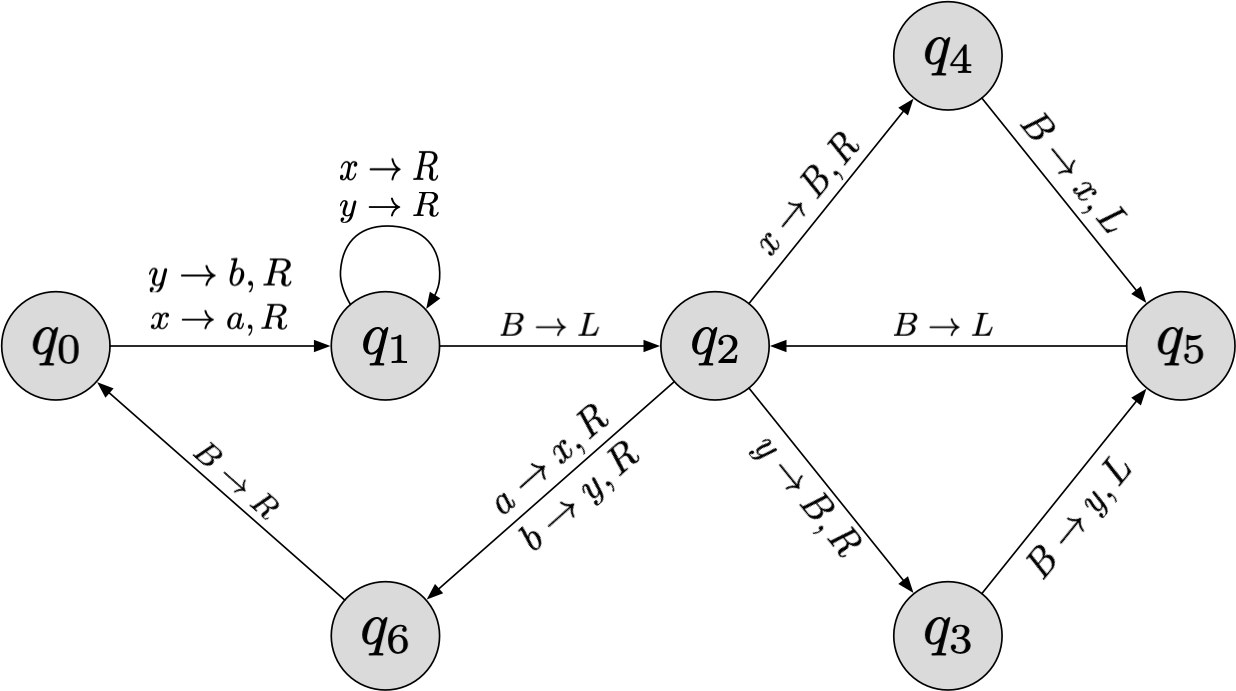
\includegraphics[scale=.5]{Q2.png}
	\end{center}
	\captionof{figure}{Turing Machine that puts blank symbol between each and every character in tape \\ ($B \rightarrow L$ = $B \rightarrow B, L$)}

\end{document}